
\chapter{Wave Function Collapse auf Graphen}
    In diesem Kapitel wir dargestellt, wie der Wave Function Collapse Algorithmus erweitert wird, so dass die Ausgabe nicht nur auf einem Gitter, sondern auch auf Zellen mit freier Anordnung und Verteilung, einem Graphen, geschehen kann. Es wird erklärt welche Aspekt des Algorithmus angepasst werden. Desweiteren wird ein neues Konzept names \textit{Heat} eingeführt, womit die Erfolgsquote des Algorithmus für spezielle Graphen verbessert wird, indem Überlappungsregeln abgeschwächt werden, wodurch die Ausgabe eine geringere Ähnlichkeit zum Beispiel haben kann.
    
    
    \section{Beschränkung des Algorithmus und Idee zur Erweiterung}
        Die ursprüngliche Form des Wave Function Collapse nimmt ein 2D Pixelmuster oder Tilesets als Beispiel und produziert daraus wieder 2D Muster. Pixel liegen stets auf einem Gitter. Bei Tilesets ist die grafische Gestaltung des Tiles zwar uneingeschränkt, dennoch sind die Tiles selbst quadratisch. Dies schränkt die Gestaltung des Inhalts der Tiles in sofern ein, dass die Kanten zu anderen Kanten passen müssen. Auch bei 3D Beispielen werden die Modelle in blockförmige Bauteile zerschnitten, damit der Algorithmus auf einem 3D Gitter von Würfeln arbeiten kann.
        
        Gitter bringen bestimmte Vorteile durch ihre Struktur mit sich. Die Benachbarung von Zellen ist implizit aus dem Gitter erkennbar, die Nachbarzellen befinden sich stets in festen Abständen in die vier Himmelsrichtungen im 2D Gitter und entlang der drei Achsen, also 6 Richtungen, im 3D Gitter. Die Überlappungsregeln aus dem Beispiel können also direkt von dem einem Gitter auf das andere übertragen werden. Der Nachteil solcher Gitter ist, dass die Ausgabe im Ganzen Artefakte des Gitter aufweist (siehe Abbildung \ref{fig:aliasing}). Nur vertikale und horizontale Linien können im Pixelgitter exakt dargestellt werden, frei geformte Kurven oder organische Strukturen lassen sich nur durch Annäherung darstellen und es kann zu Aliasing kommen.
        
        \begin{figure}[H]
    \centering
    \begin{subfigure}{0.18\textwidth} 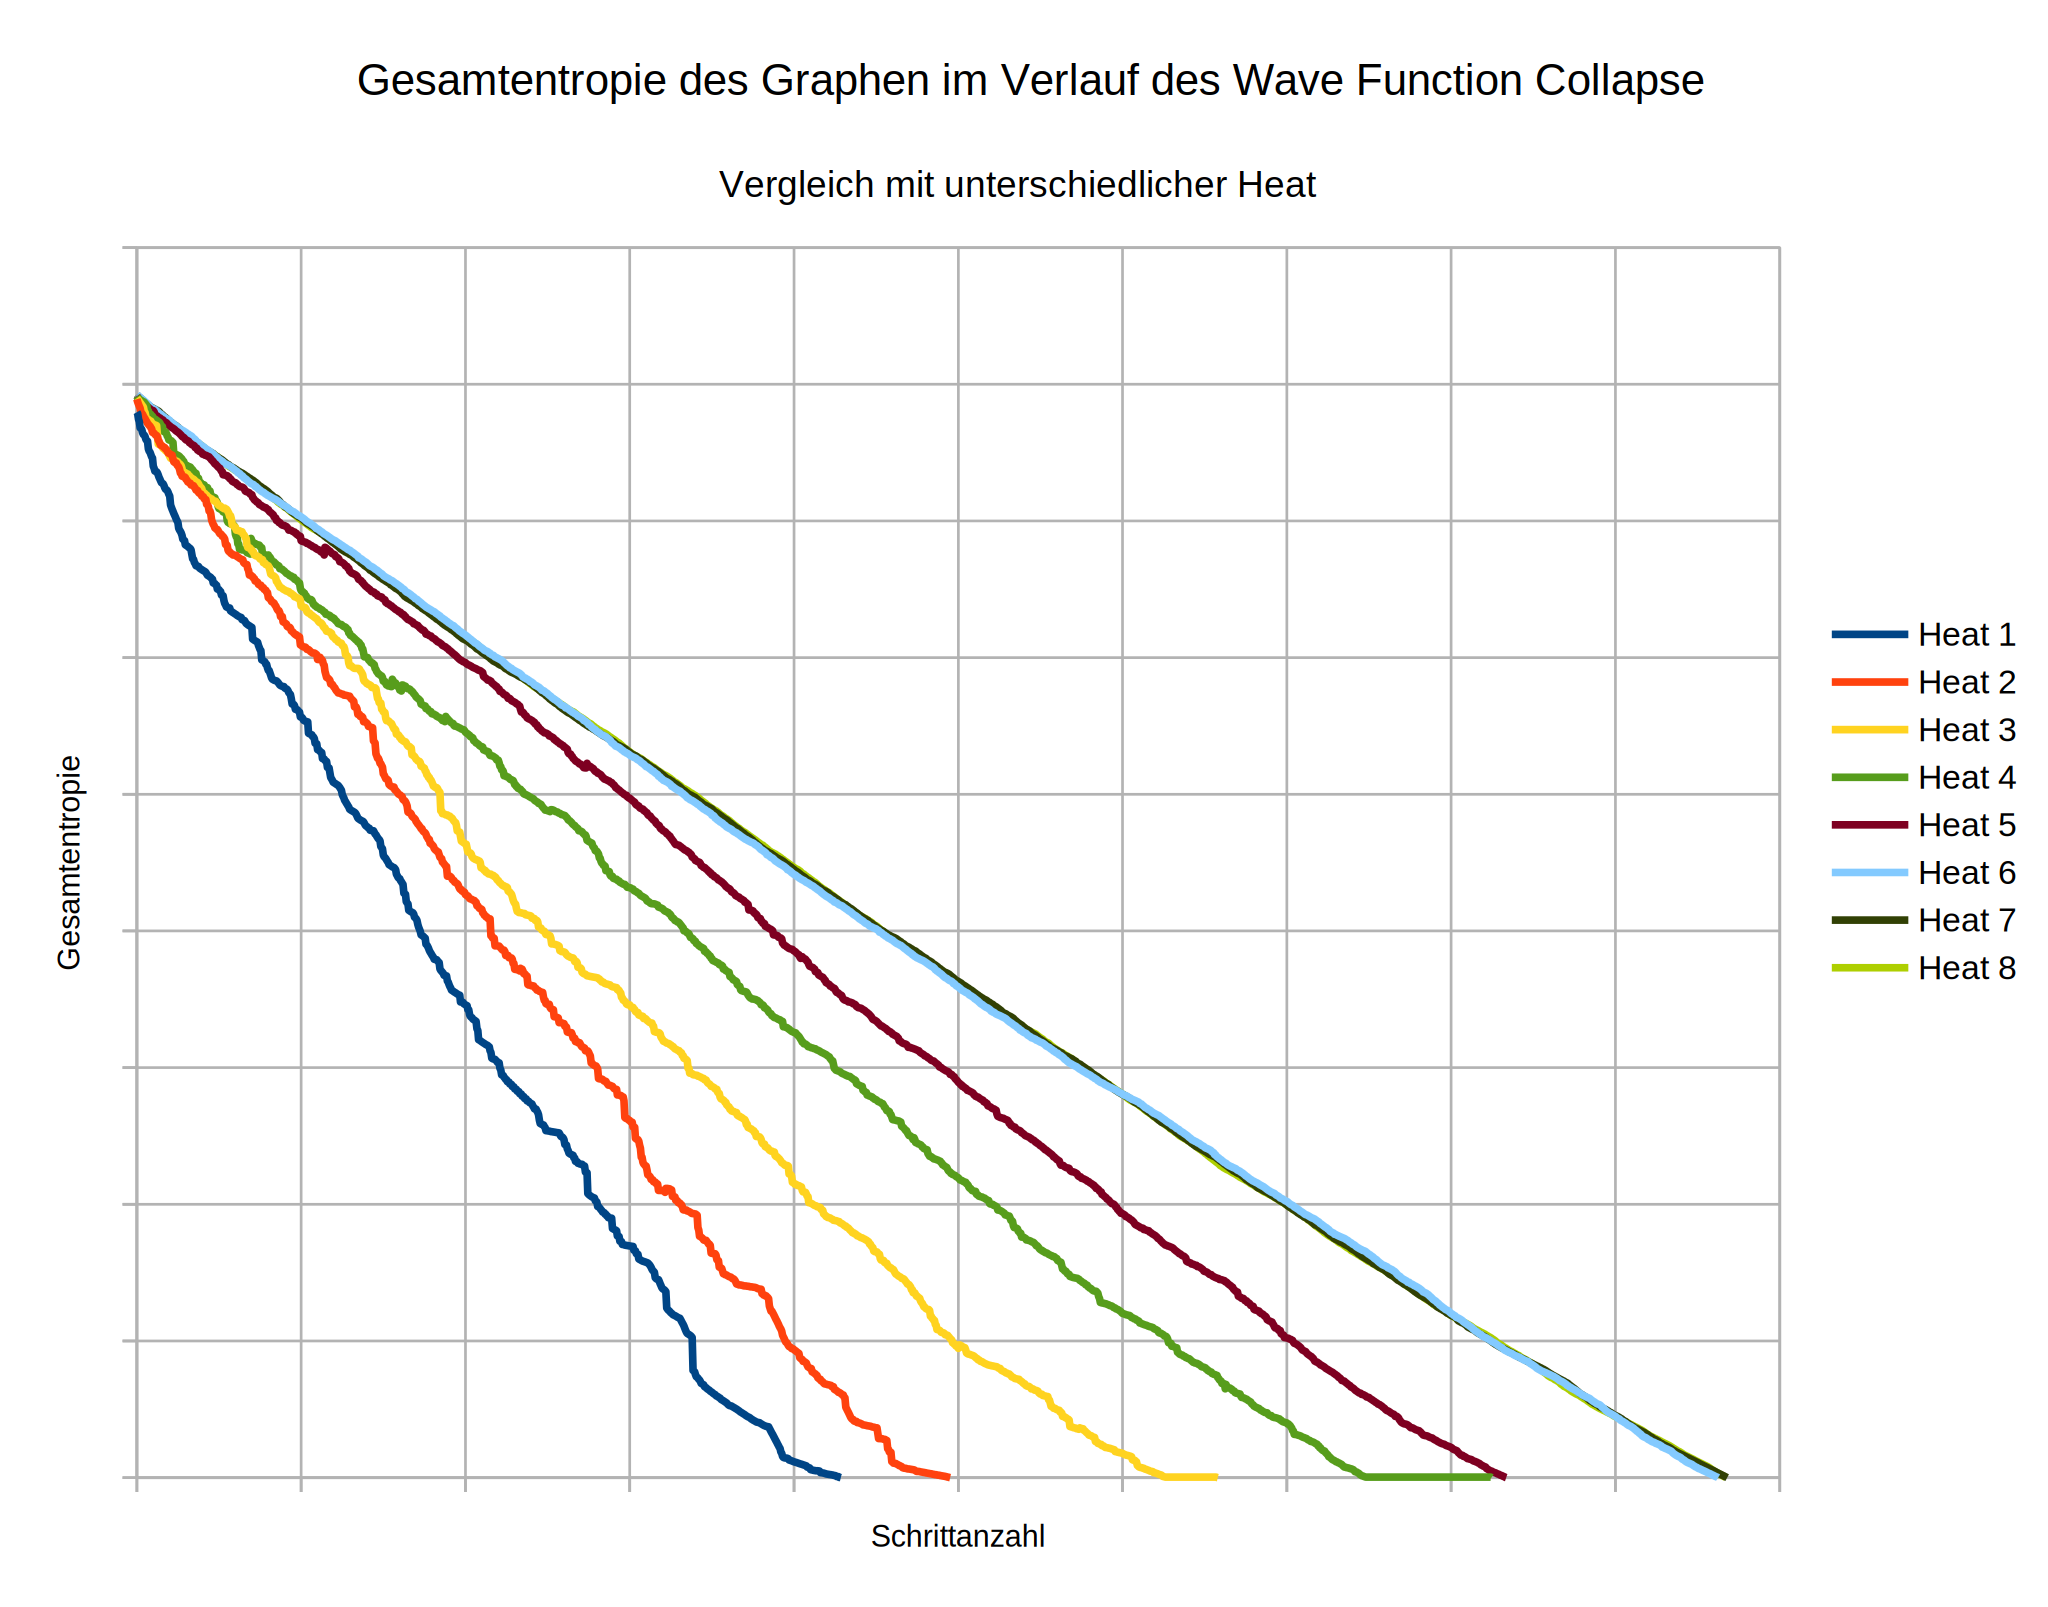
\includegraphics[width=\linewidth]{data/townscaper_grid/1.png} \caption{} \end{subfigure}
    \begin{subfigure}{0.18\textwidth} \includegraphics[width=\linewidth]{data/townscaper_grid/2.png} \caption{} \end{subfigure}
    \begin{subfigure}{0.18\textwidth} \includegraphics[width=\linewidth]{data/townscaper_grid/3.png} \caption{} \end{subfigure}
    \begin{subfigure}{0.18\textwidth} \includegraphics[width=\linewidth]{data/townscaper_grid/4.png} \caption{} \end{subfigure}
    \begin{subfigure}{0.18\textwidth} \includegraphics[width=\linewidth]{data/townscaper_grid/5.png} \caption{} \end{subfigure}
    
    \caption{
        Generierung eines Teils des Gitters für Townscaper \cite{stalberg_grid}. (a) Punkte werden generiert. (b) Triangulierung. (c) Kanten werden gelöscht, so dass Vierecke entstehen. (d) die Vierecke werden geviertelt. (e) Position der Knoten wird aufgelockert, so dass die Winkel zwischen Kanten gleichmäßiger sind.
    }
    \label{fig:townscaper_grid}
\end{figure}
        
        Im Kern des Wave Function Collapse wird geprüft, dass nur Zustände gewählt werden, die mit der Ausgabe bis dahin überlappen könnten. Die möglichen Überlappungen hängen dabei von der Richtung zwischen den Zellen ab. In einem Gitter kann jede Richtung zu einer Nachbarzelle aus dem Beispiel extrahiert werden. Wird die Anordnung und Benachbarung der Zellen nun aber vom Gitter gelöst, so ist es nicht mehr garantiert, dass die Richtungen zwischen Nachbarzellen auch im Beispiel existieren, stattdessen müssen die tatsächlichen Richtung auf eine der extrahierbaren Richtungen übersetzt werden. Danach kann der Algorithmus wie zuvor mit den Überlappungsregeln arbeiten um nun den Graphen zu befüllen.
    
    
    \section{Von Gittern zu Graphen}
        Ursprünglich arbeit Wave Function Collapse nur auf Gittern \cite{merrel, gumin}. Der Schritt zum Graphen als Fundament für die Ausgabe des Algorithmus ist naheliegend, da Gitter eine spezielle Art von Graphen darstellen. Im Umfang dieser Arbeit werden aber auch nicht alle Arten von Graphen betrachtet. Da jede Kanten eines Gitters zuvor eine lokale Benachbarung dargestellt haben und die Regelextraktion nur lokal arbeitet, beschränkt sich diese Arbeit nur auf Graphen in denen Kanten auch primär einen Knotenpunkt mit den Knotenpunkten in einem lokalen Umfeld verbindet. Der Algorithmus kann auch auf anderen Arten von Graphen angewendet werden, doch können daraus neue oder unerwartete Effekte hervortreten, die wiederum anderen Lösungswege benötigen.
        
        Ein Gitter enthällt implizit Information über Benachbarung und Position jeder Zelle. Diese Informationen werden bei Graphen explizit angegeben. Dazu kommt, dass je nach Anordnung nun nicht nur die Richtung zur Nachbarzelle, sondern auch deren Abstand und die Anzahl an Nachbarzellen variieren kann. Dieser Aspekt ist von Vorteil für die Gestaltung der Ausgabe, da nun beliebige Strukturen und Formen genutzt werden können. Doch der Nachteil ist, dass das Beispiel und die daraus extrahierten Regeln vom Algorithmus nicht mehr eins zu eins angewendet werden können.
        
        
        
    \section{Heat}
        In einem 2D Gitter sind die Nachbarn jeder Zelle per Definition in festen Richtungen und Abständen zu finden. Bei Graphen ist diese Anordnung frei. Während des Algorithmus werden die möglichen Zustände von Nachbarzellen auf Überlappung geprüft. Ein Zustand einer Zelle ist möglich, wenn er mit mindestens einem Zustand jeder Nachbarzelle überlappen kann. Die Überlappung zweier Zustände hängt von der Richtung zwischen den Umfeldern der Zustände abhängt ab. Das heißt, dass für den Nachbar im Norden einer Zelle nur die Überlappung der Zustände im Norden relevant ist. Die Richtung zu einer Nachbarzelle auf einem Graphen wird als der Vektor vom Mittelpunkt der Zelle zum Mittelpunkt der Nachbarzelle definiert. Der wichtigste Unterschied ist, dass die Richtung nun nicht mehr, wie auf dem Gitter, auf die Himmelsrichtungen beschränkt ist. 
        
        Es ist nicht möglich Regeln für eine beliebige Richtung aus dem Beispiel zu extrahieren, da jeder Pixel nur 8 angrenzende Pixel hat. Sieht man das Beispiel als eine Funktion an, so ist diese nicht an allen Punkten definiert. Man könnte durch Interpolation einen Mittelwert zwischen Pixeln berechnen, wenn das Bild eine kontinuierliche Funktion approximiert. Handelt es sich aber tatsächlich um eine diskrete Funktion, könnte eine Interpolation Werte ergeben die nicht Teil des Wertebereichs waren, in anderen Worten würde man Farbwerte erhalten die vorher nicht im Bild waren. Da die Ausgabe dem Beispiel ähnlich seien muss, entfällt diese Option.
        
        Es bleibt also nur die Möglichkeit, dass der tatsächlichen Richtung eine der messbaren Himmelsrichtungen zugewiesen wird. Hierfür wird die Kosinus-Ähnlichkeit berechnet (siehe Formel \ref{eq:cosine}). Ist der Wert hoch, so zeigen die Vektoren in eine ähnliche Richtung, während entgegengesetze Vektoren eine geringe Ähnlichkeit haben. Es wird die Himmelsrichtung mit der höchsten Ähnlichkeit gewählt. 
        
        \begin{figure}[H]
    \centering
    
    $$ \mathrm{similarity}(\mathbf{a},\mathbf{b}) = \frac{\mathbf{a}\cdot\mathbf{b}}{\|\mathbf{a}\|_2\,\|\mathbf{b}\|_2} $$
    
    \caption{Formel für die Kosinus-Ähnlichkeit}
    
    \label{fig:cosine}
\end{figure}
        
        Nun kann mit dieser Auswahlt weitergearbeitet werden. Der Nachbar wird als in dieser Himmelrichtung liegend behandelt und daraus ergibt sich, welche Überlappungsregeln benutzt werden. Sind die Zellen beinahe oder ausschließlich entlang der Himmelrichtungen angeordnet, dann funktioniert diese Rundung gut. Liegt eine Nachbarrichtung nun aber genau zwischen zwei Himmelrichtungen, so haben beide die gleiche Ähnlichkeit und der Algorithmus muss willkürlich eine der beiden wählen. Diese Entscheidung wird bereits vor Beginn der Generierung getroffen, was den schlechtesten Zeitpunkt dafür darstellt, da am wenigsten Information vorliegt. Um zu wissen welche Himmelrichtung bessere Ergebnisse liefert, müssten beide Optionen jeweils ausprobiert und verglichen werden. Da jede Zelle mit ihrem finalen Zustand aber jede andere Zelle beeinflussen kann, müsste jede Kombination für alle Zellen geprüft werden, was schnell unmöglich wird. Stattdessen wäre es besser die Entscheidung bis zum letzten Moment, also dann wenn eine Zelle kollabiert wird, aufzuschieben. Zu diesem Zeitpunkt hat der Algorithmus die meisten Informationen und kann dadurch einen Widerspruch besser vermeiden. Beim Kollabieren wird der Zelle immernoch ein einziger Zustand zugewiesen, wodurch implizit ebend die Himmelsrichtung, mit der der gewählte Zustand mit den Nachbarzellen überlappt, ausgewählt wird.
        \\
        \\
        \textit{Heat} gibt an wie viele Himmelrichtungen der Algorithmus für Nachbarn betrachtet. Diese wird im Umfang dieser Arbeit für alle Zellen des Graphen einheitlich gesetzt und vor Beginn der Generierung festgelegt. Damit ein Zustand nun für eine Zelle möglich ist, muss dieser mit den Zuständen der Nachbarzellen überlappen. Nun muss die Überlappung entsprechend der Heat nicht nur noch entlang einer Himmelrichtung sein, sondern es können mehrere geprüft werden, wobei es reicht wenn eine der Himmelsrichtungen eine passende Regel hat. Ein Effekt höherer Heat ist, dass Zellen mehr mögliche Zustände haben, da es für jeden Zustand mehr passende Regeln gibt; die Entropie der Zellen ist tendenziell höher als bei geringer Heat.
        
        Die Anzahl der extrahierten Himmelsrichtungen begrenzt den Wertebereich für die Heat. Jeder Benachbarung kann minimal eine und maximal alle Himmelsrichtungen zugewiesen werden. Da Wave Function Collapse zuvor auf Gittern lief, konnten die Regelextraktion optimiert werden. Die reguläre Struktur des Gitters führt dazu, dass wenn für eine Zelle $A$ der Nachbar von $A$ im Norden($A_n$) passt und der Nachbar im Westen von $A_n$ passt, dann muss auch der Nachbar von $A$ im Nordwesten passen. Somit mussten nur die Überlappungsregeln für Norden, Süden, Westen und Osten gespeichert werden. Für die Generierung auf Graphen entfällt dies. Die diagonalen Himmelsrichtungen werden explizit gespeichert und behandelt.
    
    
    
    \section{Zusammenfassung}
        Ziel dieser Arbeit ist, die Generierung des Wave Function Collapse Algorithmus auf Graphen geschehen zu lassen. Hierfür wurden drei Anpassungen dargestellt:
        \begin{enumerate}
            \item Ein Gitter gibt implizit an, wo Zellen liegen und welche Zellen benachbart sind. Diese Informationen müssen im Graphen explizit gespeichert werden. 
            \item Für Gitter genügt es bei der Regelextraktion die Himmelrichtungen entlang der Achsen zu betrachtet. Bei Graphen sollten aber auch die Diagonalen extrahiert und gespeichert werden.
            \item Die aus dem Beispiel extrahierten Überlappungsregeln können nicht wie bei Gittern direkt angewendet werden. Die für eine Nachbarzelle relevanten Regeln werden aus der tatsächlichen Richtung zu dieser berechnet. Diese Zuweisung wird mittels Heat erweitert, so dass mehr als eine Himmelsrichtung ausgewählt werden kann.
        \end{enumerate} 



\chapter{Umsetzung}
    Abbildung \ref{fig:app} zeigt einen Screenshot der, für diese Arbeit entwickelten, Anwendung, in dem die UI und eine generierte Ausgabe zusehen sind. Der Nutzer kann Beispielbilder auswählen, einen Graphen generieren und dann mittels Wave Function Collapse eine Ausgabe generieren. Der Quellcode ist hier\footnote{\url{https://github.com/MrMetube/wfc} (Stand: \today)} verfügbar.
    
    \begin{figure}[H]
    \centering
    \begin{subfigure}{0.18\textwidth} 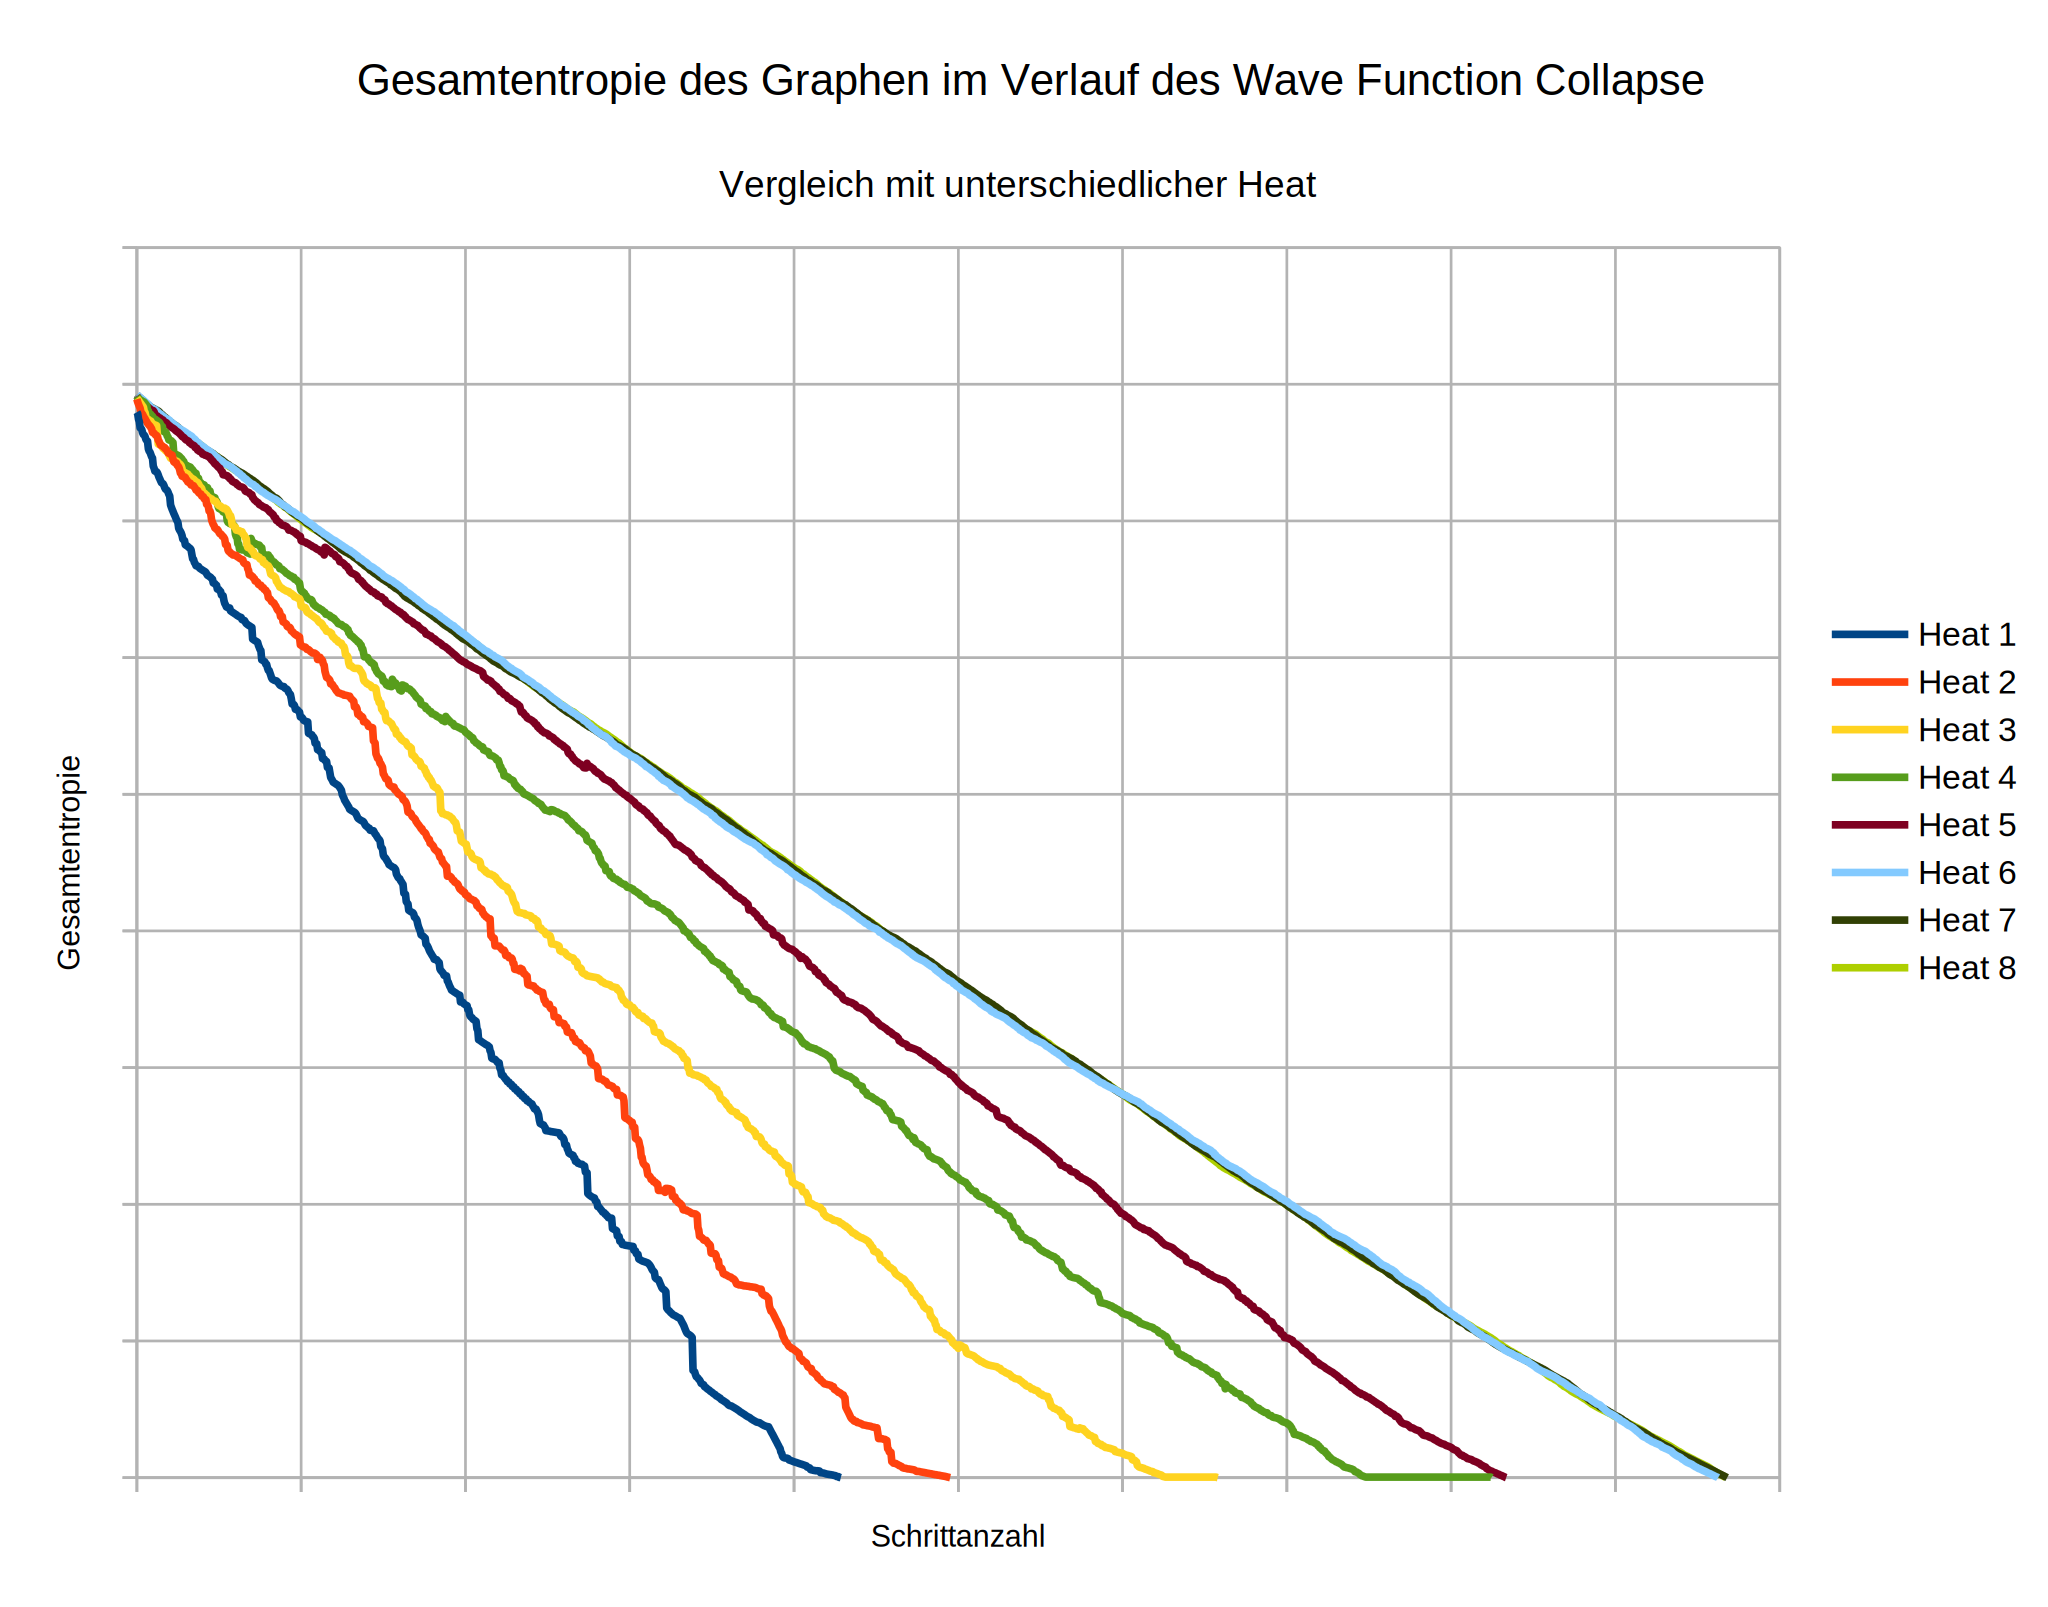
\includegraphics[width=\linewidth]{data/townscaper_grid/1.png} \caption{} \end{subfigure}
    \begin{subfigure}{0.18\textwidth} \includegraphics[width=\linewidth]{data/townscaper_grid/2.png} \caption{} \end{subfigure}
    \begin{subfigure}{0.18\textwidth} \includegraphics[width=\linewidth]{data/townscaper_grid/3.png} \caption{} \end{subfigure}
    \begin{subfigure}{0.18\textwidth} \includegraphics[width=\linewidth]{data/townscaper_grid/4.png} \caption{} \end{subfigure}
    \begin{subfigure}{0.18\textwidth} \includegraphics[width=\linewidth]{data/townscaper_grid/5.png} \caption{} \end{subfigure}
    
    \caption{
        Generierung eines Teils des Gitters für Townscaper \cite{stalberg_grid}. (a) Punkte werden generiert. (b) Triangulierung. (c) Kanten werden gelöscht, so dass Vierecke entstehen. (d) die Vierecke werden geviertelt. (e) Position der Knoten wird aufgelockert, so dass die Winkel zwischen Kanten gleichmäßiger sind.
    }
    \label{fig:townscaper_grid}
\end{figure}
    
    \section{Generierung von Graphen}
        Die Graphen auf denen der Wave Function Collapse arbeiten soll, werden in dieser Arbeit mit dem folgenden Algorithmus \ref{alg:graph_gen} generiert. Der Algorithmus nimmt als Eingabe eine Menge an Punkten, welche die Knotenpunkte des Graphen werden. Aus den Punkten wird eine Delaunay-Triangulierung erstellt. Hierfür wird der Boywer-Watson \cite{bowyer, watson} Algorithmus \ref{alg:bowyer_watson} verwendet. Danach wird das Voronoi-Diagramm zu der Triangulierung gefunden. Der duale Graph der Delaunay-Triangulierung ist das Voronoi-Diagramm, d.h. jeder Knotenpunkt des Voronoi-Diagramms entspricht einer Fläche der Triangulierung und jede Fläche im Voronoi-Diagramm entspricht einem Knotenpunkt in der Triangulierung. Die Kanten der Dreiecke geben an, welche Zellen aneinander angrenzen, während die Voronoi-Zellen die Form einer Zelle für die Darstellung geben. In Abbildung \ref{fig:graph_examples} sind einige Beispiele von generierten Graphen dargestellt. Es ist zuerkennen, dass regelmäßige Gitter nur eine spezielle Form von Graphen darstellen. Daher können regelmäßige Gitter und unregelmäßige Graphen in einem Graphen kombiniert werden.
        
        \begin{algorithm}
    \caption{Generierung eines Graphen}
    \label{alg:graph_gen}
        
    \begin{enumerate}
    \item Erstelle eine Menge an Punkten
    
    \item Generiere die Delaunay-Triangulierung der Punkte
    \subitem Die Ecken und Kanten aller Dreiecke bilden den Graphen
        
    \item Erstelle die Voronoi-Zellen aus der Triangulierung \begin{enumerate}
        \item Finde alle Dreiecke, die einen Punkt teilen
        \item Die Schwerpunkte dieser Dreiecke sind die Eckpunkte der Zelle
        \item Verbinde die Eckpunkte der Zelle mit Kanten
        \item Begrenze die Voronoi-Zellen auf den gewünschten Bereich 
        \subitem siehe Abbildung \ref{fig:voronoi_clipping}
        \end{enumerate}
    \end{enumerate}
        
\end{algorithm}
        
        \begin{algorithm}
    \caption{Bowyer-Watson Algorithmus \cite{bowyer, watson}}
    \label{alg:bowyer_watson}
        
    \begin{enumerate}
        \item Geben sei eine Menge an Punkte
        \item Erstelle das Super-Dreieck so dass jeder Punkt innerhalb liegt
        
        \item Füge jeden Punkt schrittweise in die Triangulierung ein: \begin{enumerate}
            \item Finde die Dreiecke in dessen Umkreis der Punkt liegt
            \subitem Ist der Punkt innerhalb des Umkreises kann dieses Dreieck nicht zur finalen Triangulierung gehören
            \item Sammel alle Kanten dieser Dreiecke
            \subitem Kommt eine Kante nur einmal vor, ist sie Teil der Hülle dieser Dreiecke
            \subitem Alle anderen Kanten sind innerhalb dieser Hülle, da sich zwei Dreiecke diese Kante teilen
            \item Erstelle eine neue Kante zum eingefügten Punkt für jede Ecke der Hülle
            \item Erstelle neue Dreiecke aus diesen Kanten und der Hülle
            \item Füge die neuen Dreiecke in die Triangulierung ein
        \end{enumerate}
        
        \item Enferne alle Dreiecke die eine Kanten mit dem Super-Dreieck teilen
        \item Die Ecken und Kanten aller Dreiecke bilden den Graphen
        \subitem Jede Ecke wird der Mittelpunkt einer Voronoi-Zelle
        \subitem Die Kanten zeigen welche Zellen benachbart sind
    \end{enumerate}
        
\end{algorithm}
        
        \pagebreak
        
        \begin{figure}[H]
    \centering
    \begin{subfigure}{0.18\textwidth} 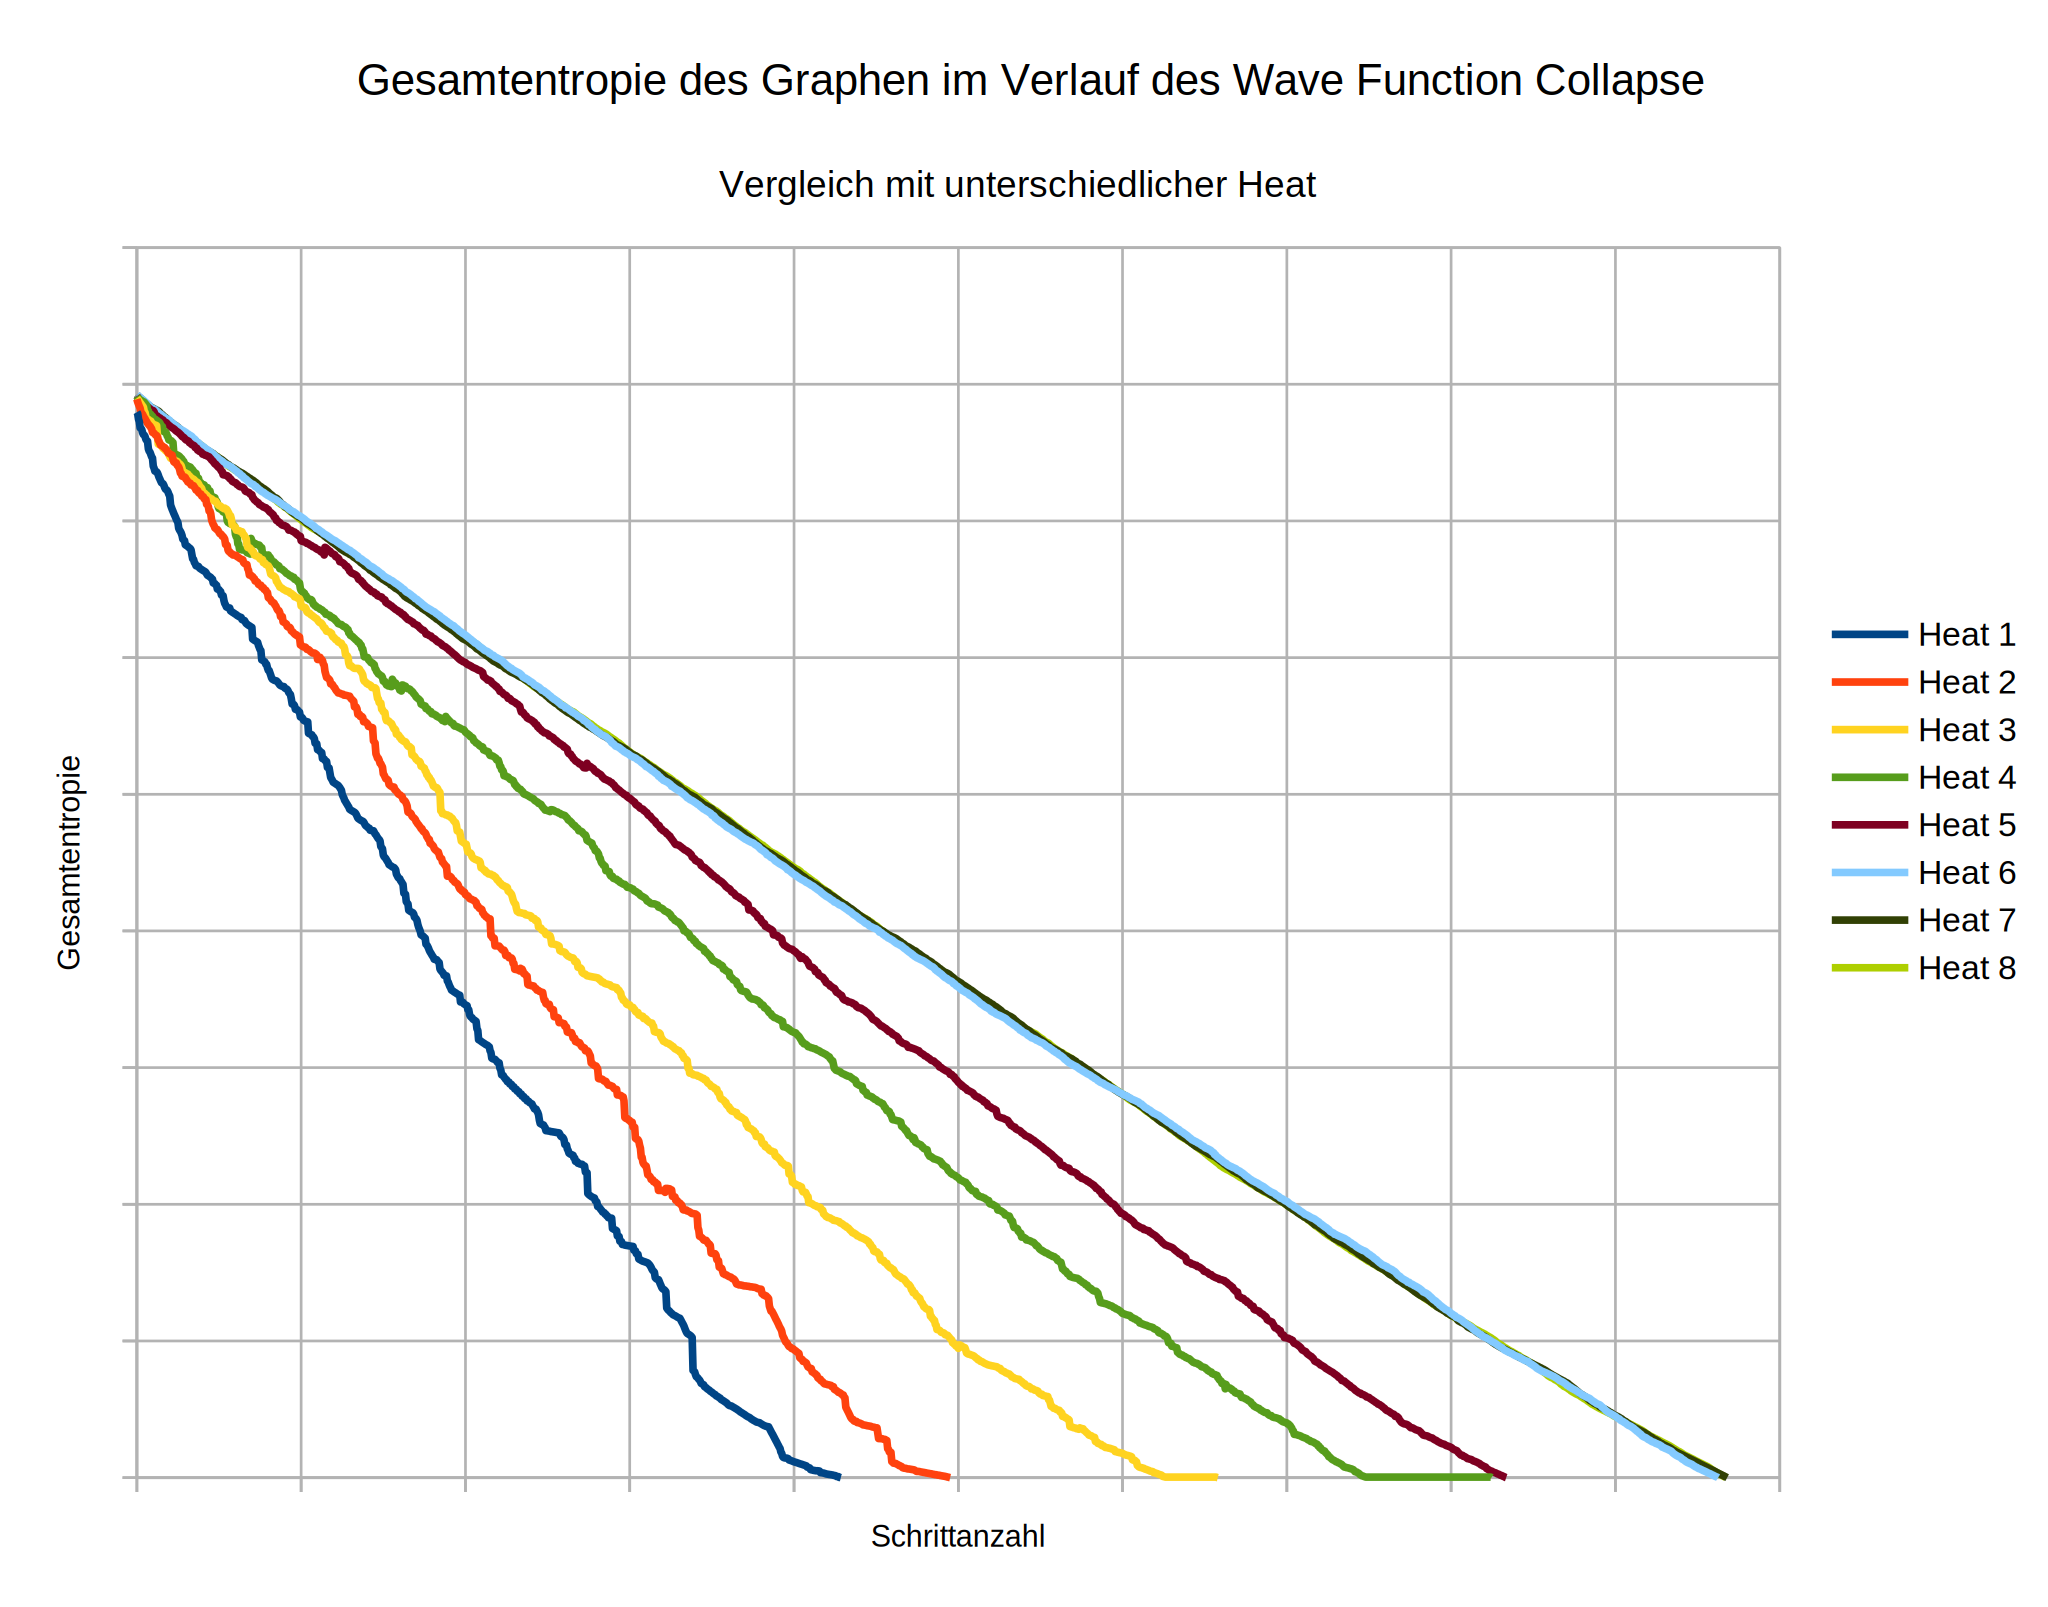
\includegraphics[width=\linewidth]{data/townscaper_grid/1.png} \caption{} \end{subfigure}
    \begin{subfigure}{0.18\textwidth} \includegraphics[width=\linewidth]{data/townscaper_grid/2.png} \caption{} \end{subfigure}
    \begin{subfigure}{0.18\textwidth} \includegraphics[width=\linewidth]{data/townscaper_grid/3.png} \caption{} \end{subfigure}
    \begin{subfigure}{0.18\textwidth} \includegraphics[width=\linewidth]{data/townscaper_grid/4.png} \caption{} \end{subfigure}
    \begin{subfigure}{0.18\textwidth} \includegraphics[width=\linewidth]{data/townscaper_grid/5.png} \caption{} \end{subfigure}
    
    \caption{
        Generierung eines Teils des Gitters für Townscaper \cite{stalberg_grid}. (a) Punkte werden generiert. (b) Triangulierung. (c) Kanten werden gelöscht, so dass Vierecke entstehen. (d) die Vierecke werden geviertelt. (e) Position der Knoten wird aufgelockert, so dass die Winkel zwischen Kanten gleichmäßiger sind.
    }
    \label{fig:townscaper_grid}
\end{figure}
        
        \pagebreak
        
        \begin{figure}[H]
    \centering
    \begin{subfigure}{0.18\textwidth} 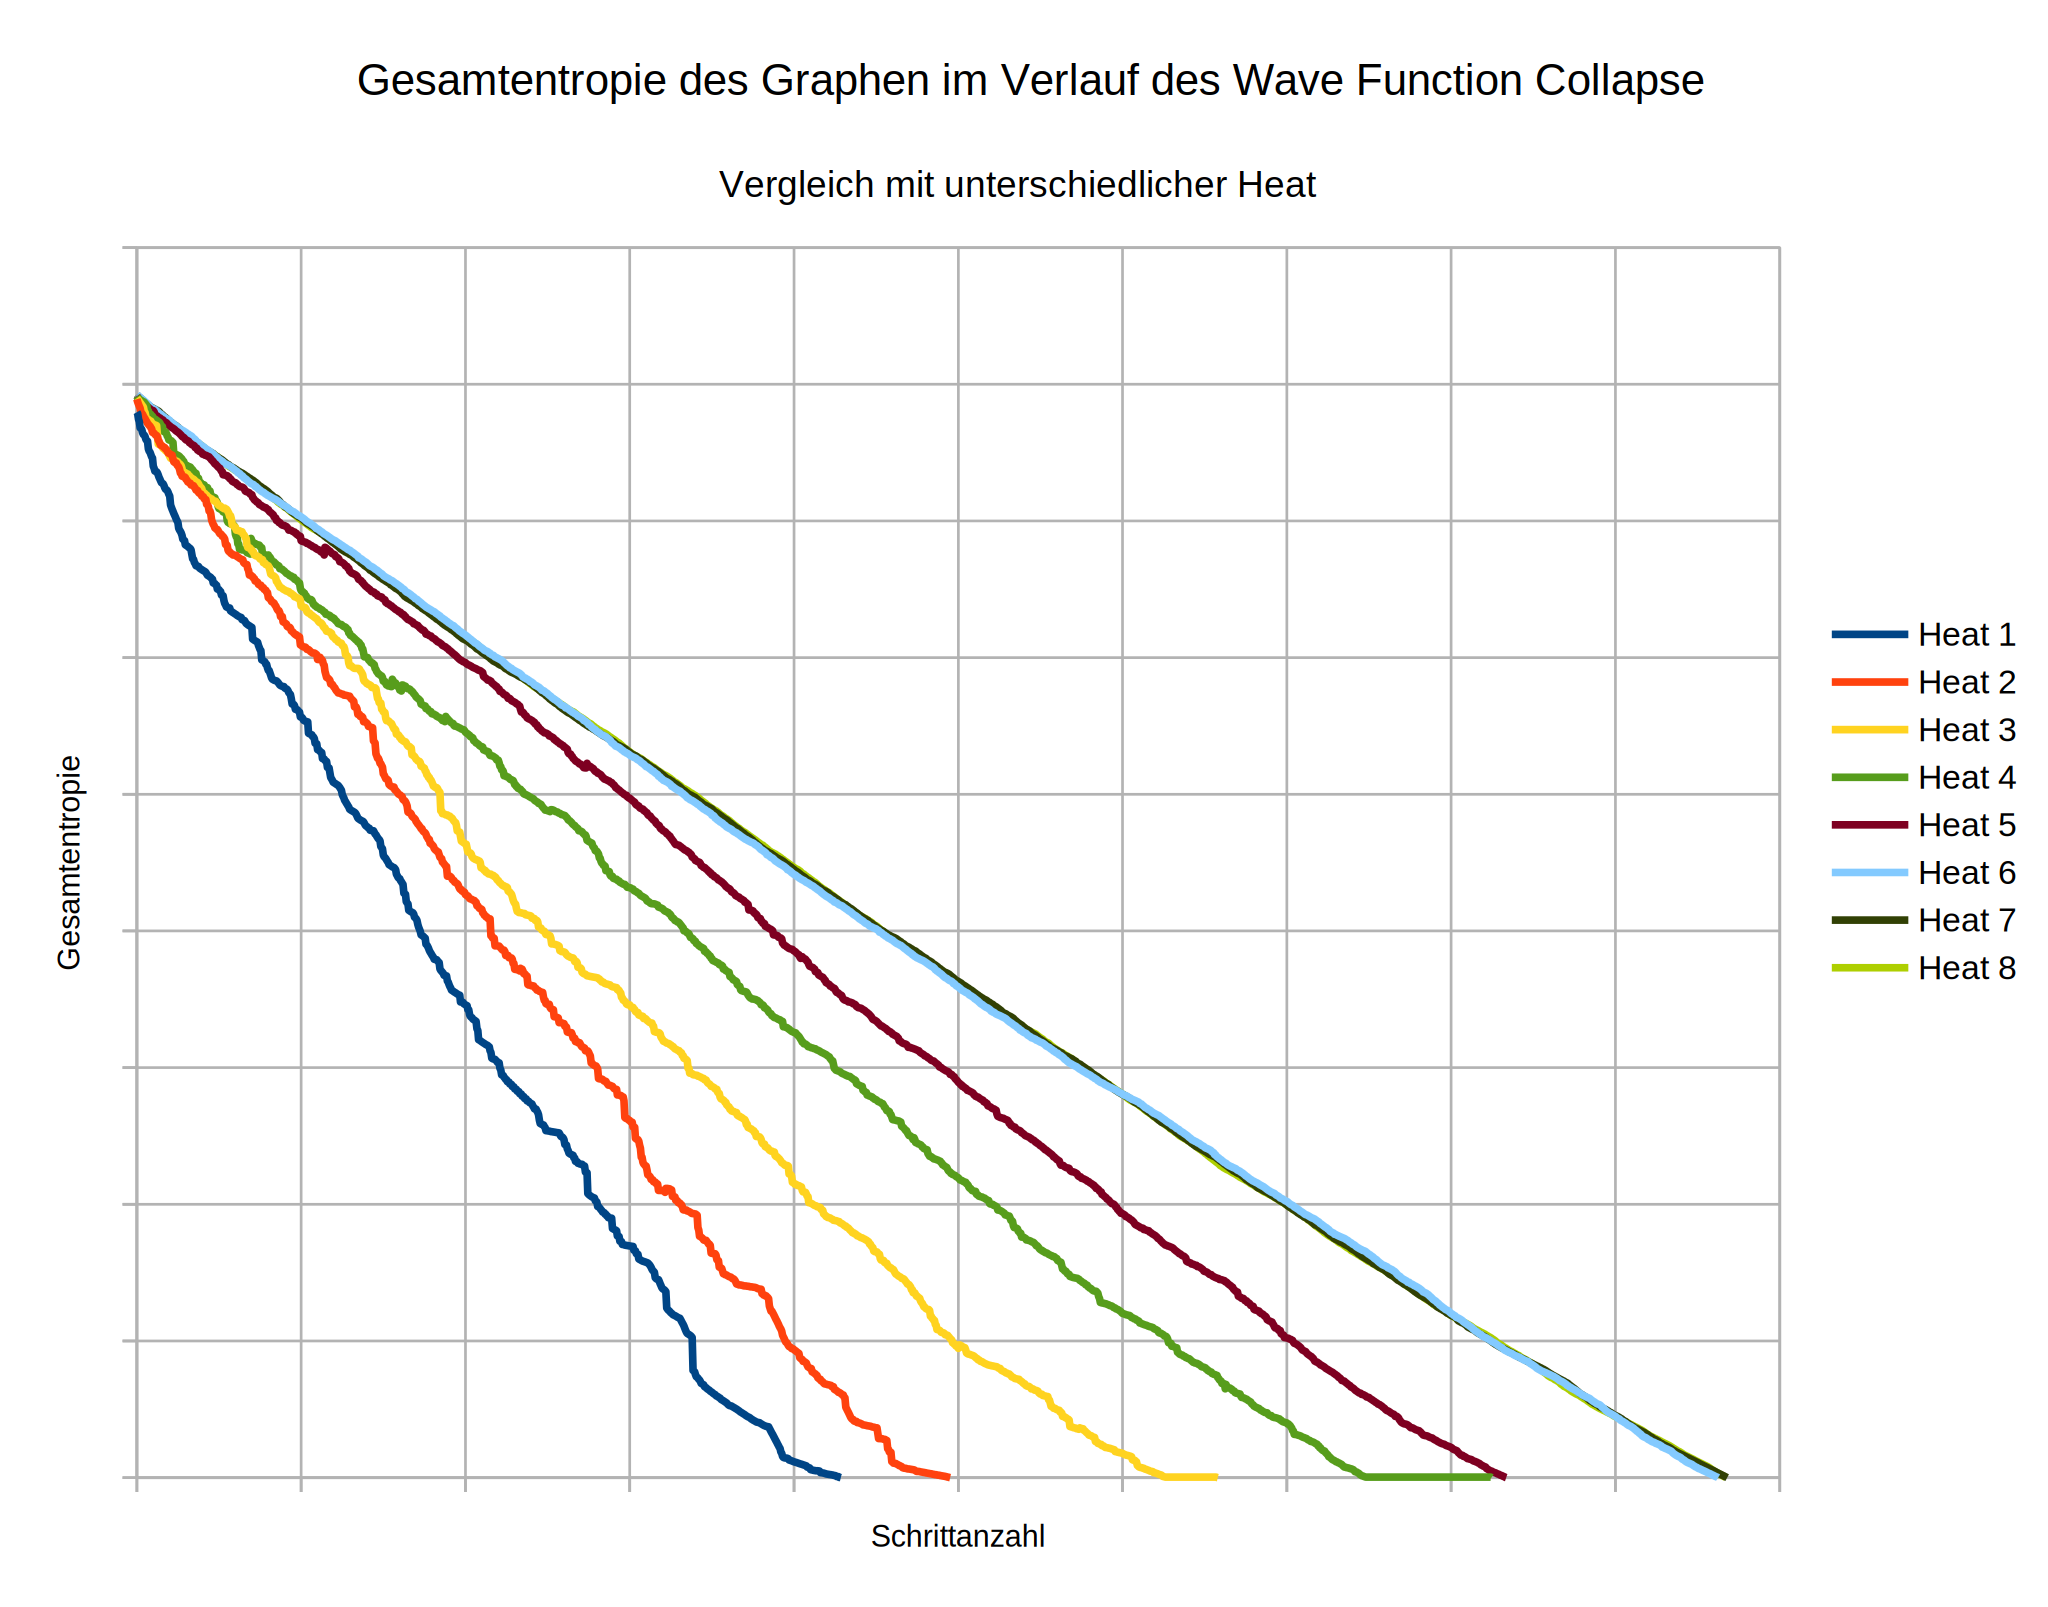
\includegraphics[width=\linewidth]{data/townscaper_grid/1.png} \caption{} \end{subfigure}
    \begin{subfigure}{0.18\textwidth} \includegraphics[width=\linewidth]{data/townscaper_grid/2.png} \caption{} \end{subfigure}
    \begin{subfigure}{0.18\textwidth} \includegraphics[width=\linewidth]{data/townscaper_grid/3.png} \caption{} \end{subfigure}
    \begin{subfigure}{0.18\textwidth} \includegraphics[width=\linewidth]{data/townscaper_grid/4.png} \caption{} \end{subfigure}
    \begin{subfigure}{0.18\textwidth} \includegraphics[width=\linewidth]{data/townscaper_grid/5.png} \caption{} \end{subfigure}
    
    \caption{
        Generierung eines Teils des Gitters für Townscaper \cite{stalberg_grid}. (a) Punkte werden generiert. (b) Triangulierung. (c) Kanten werden gelöscht, so dass Vierecke entstehen. (d) die Vierecke werden geviertelt. (e) Position der Knoten wird aufgelockert, so dass die Winkel zwischen Kanten gleichmäßiger sind.
    }
    \label{fig:townscaper_grid}
\end{figure}
        
        Es ist normal, dass ein solches Voronoi-Diagramm an den Rändern Zellen ergeben kann die auf einer Seite offen sind, weil die Kanten zwischen den Ecken der Zelle, den Umkreismittelpunkten, keinen Schnittpunkt haben. Für die Darstellung werden solche Zellen so angepasst, dass ihre Fläche innerhalb eines gewünschten Bereichs liegt(siehe Abbildung \ref{fig:voronoi_clipping}). Unendlichgroße Flächen lassen sich schlecht rendern. Es wird geprüft, ob ein Eckpunkt der Voronoi-Zelle außerhalb des gewählten Bereichs liegt. Für solche Eckpunkte wird der Schnittpunkt von der Kante mit dem Bereich gefunden. Der Schnittpunkt ersetzt den Eckpunkt. Dies geschieht so lange bis alle Eckpunkte einer Zelle innerhalb oder auf dem Rand des Bereichs liegen.
    
        Nun liegt eine Graph vor, mit dem der Wave Function Collapse Algorithmus arbeiten kann. Die Knoten und Kanten der Triangulierung geben die Anordnung und Benachbarung der Zellen an, während die Voronoi-Zellen die Form jeder Zelle für die Darstellung benutzt werden können.
        
    \section{Phasen des Algorithmus und Backtracking}
        Der Algorithmus \ref{alg:wfc_back} generiert die Ausgabe schrittweise. Ein \textit{Schritt} besteht aus vier Phasen: Search, Pick, Observe und Propagate. Schritte geschehen nacheinander und könne nur eine Zelle oder bis hin zu alle Zellen anpassen. Der Algorithmus führt Schritt aus, bis jede Zelle kollabiert ist oder ein Widerspruch gefunden wurde.
        
        
        Zu Beginn werden die Zellen mit der geringsten Entropie gesucht. Es ist möglich, dass mehrere Zellen die gleiche Entropie haben. Aus der Menge an gefundenen Zellen wird in diesem Fall in der Pick-Phase eine Zelle zufällig ausgewählt. In der Observe-Phase wird ein Zustand aus der Superposition der gewählten Zelle zufällig ausgewählt und die Zelle wird in diesen Zustand kollabiert. Die anderen Zustände werden entfernt, was Einfluss auf die Nachbarzellen haben kann. Die Wahrscheinlichkeit eines Zustands, gewählt zu werden, hängt von dessen Häufigkeit im Beispiel ab. Danach beginnt die Propagate-Phase. Eine Liste aller geänderten Zellen wird mit der observierten Zelle initialisiert. Jede Zelle in der Liste wird einzeln entfernt und wie folgt bearbeitet. Alle Nachbarzellen der betrachten Zellen prüfen, welche ihrer Zustände mit keinem der Zustände der betrachteten Zellen noch überlappen. Diese Zustände werden entfernt und jede Nachbarzelle die sich so verändert hat, wird der Liste angefügt. Sollte dabei auch der letzte mögliche Zustand einer Zelle unmöglich gewurden sein, so wurde ein Widerspruch erreicht. Diese Phase dauert so lange, bis die Liste leer ist, sich also keine Zellen mehr verändern.
        
        \begin{figure}[H]
    \centering
    \begin{minipage}{\linewidth}
        \rule{\linewidth}{0.4pt}
        
        \begin{enumerate}
            \item Führe den nächsten \textbf{Schritt} aus: \begin{enumerate}
                \item \textbf{Search}: Finde die Zellen mit der geringsten Entropie \begin{enumerate}
                    \item Sind alle Zellen kollabiert? $\rightarrow$ \textbf{Done}
                    \item Erstelle ein Liste der gefundenen Zellen
                \end{enumerate}
                
                \item \textbf{Pick}: Wähle eine Zelle aus \begin{enumerate}
                    \item Ist die Liste der Zellen leer? $\rightarrow$ \textbf{Backtrack}
                    \item Entferne die gewählte Zelle aus der Liste
                    \item Notiere alle möglichen Zustände der Zelle in einer Liste
                \end{enumerate}
                
                \item \textbf{Observe}: Wähle einen Zustand aus \begin{enumerate}
                    \item Entferne den gewählten Zustand aus der Liste
                    \item Kollabier die Zelle in den Zustand
                    \item Ist die Liste der Zustände leer? $\rightarrow$ \textbf{Backtrack}
                \end{enumerate}
                
                \item \textbf{Propagate}: Prüfe alle Nachbarn von geänderten Zellen \begin{enumerate}
                    \item Erstelle eine Liste zu prüfender Zellen
                    \item Füge die ausgewählte Zelle ein
                    \item Prüfe alle Nachbarzellen ob ihre Zustände noch passen
                    \item Füge die Nachbarn in die Liste ein, wenn sie sich verändert haben
                    \item Hat die Nachbarzelle keine möglichen Zustände mehr? $\rightarrow$ \textbf{Backtrack}
                \end{enumerate}
                
                \item Geh zum nächsten \textbf{Schritt}
            \end{enumerate}
            \item \textbf{Backtrack}: \begin{enumerate}
                \item Gehe zum gewünschten Schritt zurück
                \item Gehe eine Phase in dem Schritt zurück
                \item Füge alle Zustände aller Zellen, dessen Entfernungsschritt nun nach dem aktuellen Schritt liegt, wieder in die Zelle ein
            \end{enumerate}
            \item \textbf{Done}: Gib das Resultat aus
        \end{enumerate}
            
        \rule{\linewidth}{0.4pt}
    \end{minipage}
    
    \caption{Wave Function Collapse mit Backtracking}
    
    \label{fig:wfc_back}
\end{figure}
        
        Wenn der Algorithmus einen Widerspruch entdeckt, muss nicht immer alle Arbeit verworfen werden. Gerade bei größeren oder komplizierteren Mustern oder Graphen kann es sein, dass beim ersten Versuch keine Lösung gefunden wird. Wenn ein Widerspruch in einer Zelle aber nun nur von den direkten Nachbar abhängt, so ist es wahrscheinlich, dass weiter entfernte bereits gelöste Zellen dennoch kompatibel sind und nicht verworfen werden müssen. Um einen lokalen Widerspruch aufzulösen muss meistens nur lokal eine andere Entscheidung getroffen werden.
        
        Um Backtracking umzusetzen müssen mehr Informationen behalten werden als nur der Zustand des Gitters im aktuellen Schritt. Will man nun einen oder mehrere Schritte zurückgehen, muss man wissen, welche Entscheidung man zuvor bereits getroffen hat, um dessen Effekt rückgängig zu machen. Dabei genügt es nicht nur die kollabierten Zelle und den Zustand wieder zu entfernen, weil jede Zelle von mehreren Nachbarn beeinflusst wird. Die Menge der möglichen Zustände einer Zelle ist die Schnittmenge der möglichen Nachbarzuständen der Nachbarzellen. Somit kann es sein, dass ein Zustand A aus der Menge wegen mehreren Nachbarn fehlt. Nimmt man nun durch Backtracking eine dieser Beschränkungen wieder zurück, so ist es nicht offensichtlich, ob Zustand A nun wieder möglich ist, ohne alles neu zu berechnen und zu propagieren bis sich keine Zelle mehr ändert. Stattdessen kann man aber auch speichern, in welchem Schritt ein Zustand entfernt wurde. Ein Zustand wird beim Backtracken dann wieder möglich, wenn der Schritt in dem er entfernt wurde nach dem nun aktuellen Schritt liegt. Es genügt nur diesen einen Schritt pro Zustand zu speichern, da der Algorithmus selbst jeden Zustand bis auf einen pro Zelle entfernen muss, aber einen Zustand niemals in einem späteren Schritt wieder hinzufügt. In der Umsetzung wird für jede Zelle eine Liste aller Zustände gespeichert. Jeder Zustand ist entweder möglich und wurde noch nicht als entfernt markiert oder ist unmöglich und speichert den Schritt an dem er unmöglich wurde. Es wäre auch möglich einfach eine Kopie aller Zellen in jedem Schritt zu machen. Dann müssten beim Backtracken nur die alten Zellen wieder geladen werden. Der Unterschied zur anderen Methode ist dabei, dass für jeden Schritt die Zellen (oder deren Änderungen) immer wieder kopiert werden, während die benutzte Methode für jede Zelle ihre Änderungen für jeden Schritt speichert. Da ein Zustand aber nur einmal entfernt wird, muss ebend nur jeweils ein Schritt und nicht eine lange Liste aller Schritte pro Zustand gespeichert werden.
        
        Desweiteren sollen bereits getroffenen Entscheidungen, die zu einem Widerspruch führen, nicht noch einmal wiederholt werden. Die Entscheidungspunkte in der Pick- und Observe-Phase können gleich behandelt werden. Es wird jeweils eine Liste an Auswahlmöglichkeiten für später gespeichert. Die ausgewählte Zelle oder den ausgewählten Zustand werden aus der Liste entfernt. Wird gebacktrackt, so kann einfach die nächste Möglichkeit aus der Liste auswählt und entfernt werden. Der Algorithmus läuft ab dann normal weiter. Nun wurde aber eine neue Schwachstelle in den Algorithmus eingeführt. Wenn zuvor in der Search-Phase keine Zellen mehr gefunden wurden, bedeutete dies, dass alle Zellen tatsächlich kollabiert waren. Nun kann es aber sein, dass alle gefundenen Zellen ausprobiert wurde und zu einem Widerspruch geführt haben. Somit würde keine Zelle mehr wählbar sein. Auch in der Observe-Phase war es zuvor unmöglich keinen Zustand mehr auswählen zu können, da eine Zelle ohne mögliche Zustände bereits zuvor als Widerspruch identifiziert wurden wäre. In beiden Fällen wird dies wie ein Widerspruch behandelt und es muss zum Backtracking kommen. Schließlich wurden alle von diesem Schritt folgenden Entscheidungen bereits getroffen und ausgewertet und keine Lösung gefunden. Somit führt dieser Schritt zwar nicht direkt zu einem Widerspruch in einer Zelle, aber alle folgen Schritte werden irgendwann zu einem Widerspruch führen.
